\documentclass[aspectratio=169,12pt]{beamer}
% Estilo canónico para las presentaciones de Métodos Numéricos 2026-2.
\usepackage[T1]{fontenc}
\usepackage[utf8]{inputenc}
\usepackage[spanish,es-nodecimaldot]{babel}
\usepackage{lmodern}
\usepackage{amsmath,amssymb,mathtools}
\usepackage{booktabs}
\usepackage{graphicx}
\usepackage{xcolor}
\usepackage{hyperref}

\definecolor{upazul}{HTML}{003B70}
\definecolor{upazulclaro}{HTML}{EAF2F8}
\definecolor{updorado}{HTML}{C5962E}
\definecolor{upgris}{HTML}{4A5560}
\definecolor{upverde}{HTML}{167C5A}
\definecolor{uprojo}{HTML}{B33A3A}

\setbeamercolor{normal text}{fg=black,bg=white}
\setbeamercolor{structure}{fg=upazul}
\setbeamercolor{frametitle}{fg=white,bg=upazul}
\setbeamercolor{title}{fg=upazul}
\setbeamercolor{subtitle}{fg=upgris}
\setbeamercolor{block title}{fg=white,bg=upazul}
\setbeamercolor{block body}{fg=black,bg=upazulclaro}
\setbeamercolor{alerted text}{fg=uprojo}
\setbeamercolor{example text}{fg=upverde}

\setbeamerfont{title}{size=\Huge,series=\bfseries}
\setbeamerfont{subtitle}{size=\Large}
\setbeamerfont{frametitle}{size=\LARGE,series=\bfseries}
\setbeamerfont{normal text}{size=\large}
\setbeamerfont{block title}{series=\bfseries}

\setbeamertemplate{navigation symbols}{}
\setbeamertemplate{itemize item}{\color{updorado}$\blacktriangleright$}
\setbeamertemplate{itemize subitem}{\color{upazul}$\bullet$}
\setbeamertemplate{blocks}[rounded][shadow=false]

\setbeamertemplate{frametitle}{%
  \nointerlineskip
  \begin{beamercolorbox}[wd=\paperwidth,ht=0.78cm,dp=0.24cm,leftskip=0.55cm]{frametitle}
    \usebeamerfont{frametitle}\insertframetitle
  \end{beamercolorbox}}

\setbeamertemplate{footline}{%
  \leavevmode
  \hbox{%
    \begin{beamercolorbox}[wd=.82\paperwidth,ht=2.7ex,dp=1.2ex,leftskip=.5cm]{author in head/foot}
      \color{upgris}\scriptsize Métodos Numéricos 2026-2 \hspace{0.8em} | \hspace{0.8em} Universidad del Pacífico
    \end{beamercolorbox}%
    \begin{beamercolorbox}[wd=.18\paperwidth,ht=2.7ex,dp=1.2ex,rightskip=.5cm plus1fil]{date in head/foot}
      \color{upazul}\scriptsize\hfill\insertframenumber/\inserttotalframenumber
    \end{beamercolorbox}}
  \vskip0pt}

\newcommand{\concepto}[1]{\textcolor{upazul}{\textbf{#1}}}
\newcommand{\resultado}[1]{\textcolor{upverde}{\textbf{#1}}}
\newcommand{\advertencia}[1]{\textcolor{uprojo}{\textbf{#1}}}
\newcommand{\codigo}[1]{\colorbox{upazulclaro}{\strut\texttt{#1}}}
\newcommand{\fuente}[1]{\vfill\hfill{\tiny\color{upgris}#1}}


\usepackage{listings}
\lstset{language=Python,basicstyle=\ttfamily\footnotesize,columns=fullflexible,
keepspaces=true,showstringspaces=false,breaklines=true,
literate={á}{{\'a}}1 {é}{{\'e}}1 {í}{{\'i}}1 {ó}{{\'o}}1 {ú}{{\'u}}1 {ñ}{{\~n}}1}
\newcommand{\R}{\mathbb{R}}
\newcommand{\norm}[1]{\left\lVert#1\right\rVert}
\newcommand{\PiN}{\mathcal P}
\newtheorem{thm}{Teorema}
\newtheorem{lema}{Lema}
\newtheorem{defi}{Definición}
\author{Oswaldo José Velásquez Castañón}
\institute{Universidad del Pacífico}
\date{Métodos Numéricos -- 2026-2}
\title{Integración numérica}
\subtitle{Ecuaciones integrales y Montecarlo}
\begin{document}
\begin{frame}[plain]
\begin{columns}[T,onlytextwidth]
\begin{column}{.70\textwidth}
\vspace{.7cm}{\usebeamerfont{title}\color{upazul}\inserttitle\par}
\vspace{.35cm}{\usebeamerfont{subtitle}\color{upgris}\insertsubtitle\par}
\vspace{1cm}{\large\insertauthor\par}{\normalsize\insertdate\par}
\end{column}
\begin{column}{.25\textwidth}\vspace{.55cm}
\includegraphics[width=\linewidth]{UPlogo.pdf}\end{column}
\end{columns}
\end{frame}
\begin{frame}{Ruta de la clase}
\begin{itemize}
\item Escribir una ecuación diferencial como una ecuación integral de Volterra.
\item Obtener Euler y trapecio implícito mediante cuadratura.
\item Estimar integrales y esperanzas por Montecarlo.
\item Separar error de discretización, incertidumbre muestral y error de redondeo.
\end{itemize}
Aplicaciones: acumulación de capital y utilidad esperada con consumo incierto.
\end{frame}

\begin{frame}{De la derivada a la ecuación integral}
\begin{thm}
Sea $F$ continua. Una función $y\in C^1[a,b]$ satisface
\[y'(t)=F(t,y(t)),\qquad y(a)=y_0,\]
si y solo si satisface
\[\boxed{y(t)=y_0+\int_a^t F(s,y(s))\,ds.}\]
\end{thm}
\textbf{Demostración.} En un sentido se integra la ecuación y se usa la
condición inicial. En el otro, la continuidad del integrando permite aplicar
el teorema fundamental del cálculo y recuperar la derivada.
\end{frame}

\begin{frame}{La incógnita está dentro de la integral}
No basta aplicar una cuadratura a valores conocidos:
el integrando depende de la función desconocida $y$.
Definimos el operador de Volterra
\[(\mathcal Ty)(t)=y_0+\int_a^tF(s,y(s))\,ds.\]
Si $F$ es Lipschitz en su segundo argumento, con constante $L$,
\[\norm{\mathcal Ty-\mathcal Tz}_\infty\leq L(b-a)\norm{y-z}_\infty.\]
En un espacio cerrado de funciones continuas que el operador preserve,
$L(b-a)<1$ permite aplicar el teorema del punto fijo.
Es una conexión con los métodos iterativos del curso.
\end{frame}

\begin{frame}{Euler como regla del rectángulo}
En cada paso $t_j$ a $t_{j+1}=t_j+h$,
\[y(t_{j+1})=y(t_j)+\int_{t_j}^{t_{j+1}}F(s,y(s))\,ds.\]
La regla del rectángulo izquierdo da
\[\boxed{Y_{j+1}=Y_j+hF(t_j,Y_j),\qquad Y_0=y_0.}\]
Es un método explícito: el valor nuevo se obtiene con información del paso anterior.
Para la solución exacta, si $y''$ está acotada, el error local por paso es $O(h^2)$.
Bajo regularidad y Lipschitz, el error global a tiempo final fijo es $O(h)$.
\end{frame}

\begin{frame}{Trapecio implícito}
Aplicando trapecio a la integral de cada paso:
\[\boxed{Y_{j+1}=Y_j+\frac h2
[F(t_j,Y_j)+F(t_{j+1},Y_{j+1})].}\]
Ahora $Y_{j+1}$ aparece en ambos lados. En general se resuelve una ecuación
no lineal por paso; si $F$ es lineal, basta despejar.
Si $y^{(3)}$ está acotada, el error local por paso es $O(h^3)$.
Bajo las hipótesis habituales de regularidad y estabilidad, el error global es $O(h^2)$.
Para una resolución por punto fijo del paso, $hL/2<1$ es una condición suficiente.
\end{frame}

\begin{frame}{Acumulación de capital}
Un modelo hipotético de capital agregado es
\[K'(t)=I(t)-\delta K(t),\qquad K(0)=K_0,\]
con inversión exógena $I(t)=2e^{0.02t}$, depreciación $\delta=0.05$ y $K_0=10$.
La forma integral es
\[K(t)=K_0+\int_0^t[I(s)-\delta K(s)]\,ds.\]
La solución exacta para auditar el cálculo es
\[K(t)=K_0e^{-\delta t}
+\frac2{\delta+0.02}(e^{0.02t}-e^{-\delta t}).\]
El stock se mide en unidades de capital y $I$ en unidades de capital por año.
\end{frame}

\begin{frame}{Actualizaciones para el modelo de capital}
Euler:
\[K_{j+1}=(1-\delta h)K_j+hI(t_j).\]
Trapecio implícito:
\[\boxed{K_{j+1}=\frac{(1-\delta h/2)K_j+
\frac h2[I(t_j)+I(t_{j+1})]}{1+\delta h/2}.}\]
No se necesita Newton en este ejemplo, porque la ecuación es lineal en $K_{j+1}$.
Para el problema homogéneo $K'=-\delta K$, los factores de amplificación son
$1-\delta h$ y $(1-\delta h/2)/(1+\delta h/2)$.
\end{frame}

\begin{frame}{Resultados a los diez años}
La referencia exacta es $K(10)=23.6330808385$.
\begin{center}\begin{tabular}{rrrrr}\toprule
Pasos $n$&Euler&Trapecio&Error Euler&Error trapecio\\\midrule
10&23.72679769&23.63442189&$9.372\times10^{-2}$&$1.341\times10^{-3}$\\
20&23.67914866&23.63341603&$4.607\times10^{-2}$&$3.352\times10^{-4}$\\
40&23.65592218&23.63316463&$2.284\times10^{-2}$&$8.379\times10^{-5}$\\
80&23.64445398&23.63310179&$1.137\times10^{-2}$&$2.095\times10^{-5}$\\\bottomrule
\end{tabular}\end{center}
Al dividir el paso por dos, el error se reduce aproximadamente a la mitad
para Euler y a la cuarta parte para trapecio implícito.
\end{frame}

\begin{frame}{Trayectoria del capital}
\begin{center}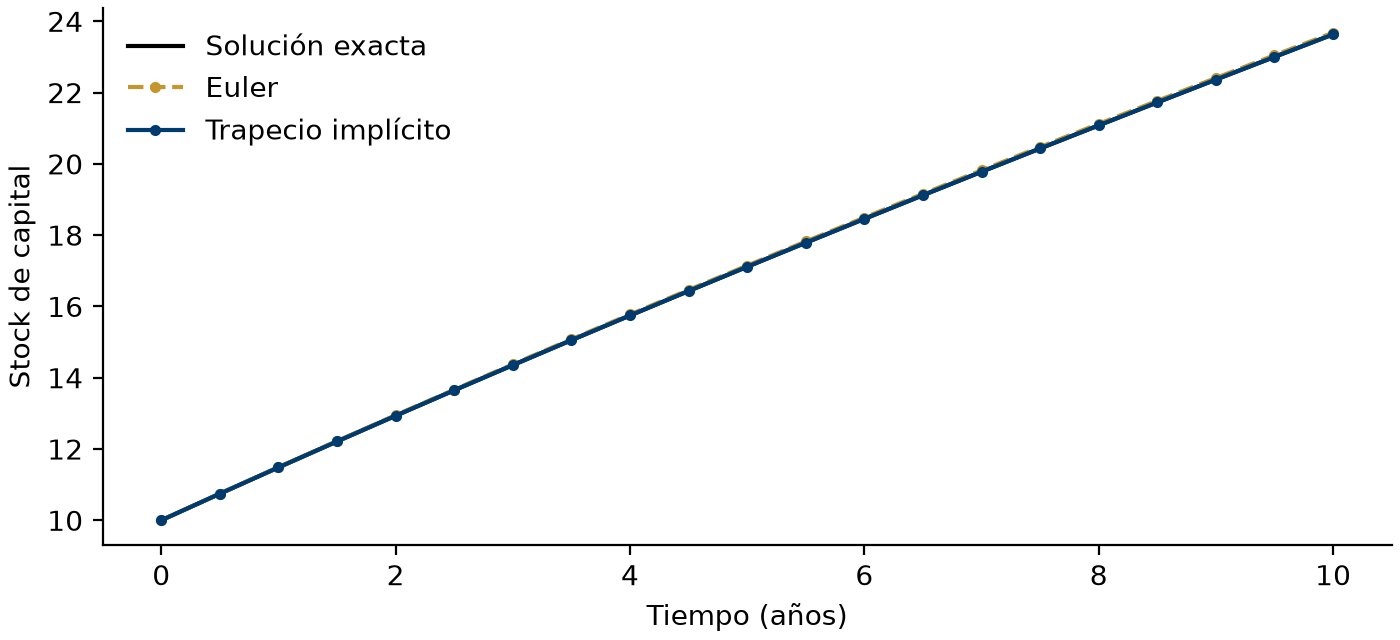
\includegraphics[height=.68\textheight]{figuras/integracion/capital.png}\end{center}
La verificación usa la solución exacta; en problemas generales se compara
refinamiento, estabilidad y residual de las ecuaciones de paso.
\end{frame}

\begin{frame}[fragile]{Implementación de la trayectoria}
\begin{lstlisting}
delta, K0, T, n = .05, 10., 10., 20
t = np.linspace(0., T, n+1)
h = T/n
I = lambda s: 2*np.exp(.02*s)
E, R = np.empty(n+1), np.empty(n+1)
E[0] = R[0] = K0
for j in range(n):
    E[j+1] = E[j] + h*(I(t[j])-delta*E[j])
    R[j+1] = ((1-delta*h/2)*R[j]
        + h/2*(I(t[j])+I(t[j+1])))/(1+delta*h/2)
\end{lstlisting}
Compruebe la condición inicial y repita con $n=10,20,40,80$.
\end{frame}

\begin{frame}{Actividad sobre la ecuación integral}
\begin{enumerate}
\item Deduzca las dos fórmulas de actualización a partir de la integral.
\item Para $K'=-\delta K$, determine cuándo el método de Euler reduce
el valor absoluto de una perturbación.
\item Distinga estabilidad numérica de preservación de capital no negativo.
\end{enumerate}
Para Euler, $|1-\delta h|<1$ equivale a $0<\delta h<2$.
Para preservar positividad del problema homogéneo basta $0\leq\delta h\leq1$.
Son condiciones distintas.
\end{frame}

\begin{frame}{Montecarlo para una integral definida}
Si $U\sim\operatorname{Unif}[a,b]$,
\[I(f)=\int_a^b f(x)\,dx=(b-a)\mathbb E[f(U)].\]
Con $U_1,\ldots,U_N$ independientes e idénticamente distribuidos,
\[\boxed{\widehat I_N=\frac{b-a}{N}\sum_{i=1}^N f(U_i).}\]
Los nodos son aleatorios. Podemos aplicarlo cuando evaluamos una función
o cuando simulamos una variable económica cuyo valor esperado nos interesa.
\end{frame}

\begin{frame}{Ley de los grandes números}
\begin{thm}
Sean $X_i=g(Z_i)$ independientes e idénticamente distribuidas.
Si $\mathbb E|X_1|<\infty$, entonces
\[\overline X_N=\frac1N\sum_{i=1}^N X_i\longrightarrow\mathbb E[X_1]
\quad\text{casi seguramente}.\]
\end{thm}
La ley asegura convergencia; no establece un error determinista para una muestra finita.
Si las simulaciones están correlacionadas, las fórmulas de varianza independientes
que siguen no se aplican directamente.
\end{frame}

\begin{frame}{Varianza y velocidad de Montecarlo}
Si $\operatorname{Var}(X_i)=\sigma_X^2<\infty$ y las muestras son independientes,
\[\mathbb E[\overline X_N]=\mathbb E[X],\qquad
\operatorname{Var}(\overline X_N)=\frac{\sigma_X^2}{N}.\]
\textbf{Demostración.} La esperanza es lineal y las covarianzas cruzadas se anulan.
El error cuadrático medio de la media, al ser insesgada, es $\sigma_X^2/N$.
Su raíz disminuye como $N^{-1/2}$.
Para reducir esa escala de error por diez se necesitan cien veces más muestras.
\end{frame}

\begin{frame}{Error estándar e intervalo asintótico}
Con $N\geq2$,
\[s_N^2=\frac1{N-1}\sum_{i=1}^N(X_i-\overline X_N)^2,\qquad
\widehat{SE}=\frac{s_N}{\sqrt N}.\]
Bajo independencia y varianza finita no nula, el teorema central del límite
motiva, para $N$ grande,
\[\overline X_N\ \pm\ 1.96\,\widehat{SE}.\]
La cobertura aproximada es $95\%$ en repeticiones del procedimiento.
No es una cota determinista para el error de una realización.
Para la integral uniforme se multiplica la media y su error estándar por $b-a$.
\end{frame}

\begin{frame}{El mismo problema de utilidad esperada}
Retomamos $C=e^{\mu+\sigma Z}$, $Z\sim N(0,1)$, $\mu=0.5$, $\sigma=0.4$,
y $u(C)=-1/C$.
\[EU=\mathbb E[-e^{-\mu-\sigma Z}]=-e^{-\mu+\sigma^2/2}.\]
La identidad se obtiene completando el cuadrado en la densidad normal:
\[-\frac{z^2}{2}-\sigma z=-\frac{(z+\sigma)^2}{2}+\frac{\sigma^2}{2}.\]
La esperanza exacta es $-0.657046819815$.
También se puede calcular con ocho nodos de Gauss--Hermite.
\end{frame}

\begin{frame}[fragile]{Montecarlo en Python}
\begin{lstlisting}
rng = np.random.default_rng(20262)
N = 100000
z = rng.standard_normal(N)
x = -np.exp(-(.5 + .4*z))
media = x.mean()
se = x.std(ddof=1)/np.sqrt(N)
intervalo = (media-1.96*se, media+1.96*se)
print(media, se, intervalo)
\end{lstlisting}
La semilla permite reproducir el experimento. No elimina el error muestral.
\texttt{ddof=1} utiliza el denominador $N-1$ en la varianza muestral.
\end{frame}

\begin{frame}{Simulación reproducible: resultados}
\small
Se usan prefijos de la misma muestra, generada con semilla 20262:
\begin{center}\begin{tabular}{rrrr}\toprule
$N$&Media&Error estándar&Error absoluto observado\\\midrule
100&$-0.6815824807$&0.0299414396&0.0245356608\\
1000&$-0.6666164684$&0.0089781239&0.0095696486\\
10000&$-0.6561036400$&0.0027436853&0.0009431798\\
100000&$-0.6559918129$&0.0008605459&0.0010550070\\\bottomrule
\end{tabular}\end{center}
Para $N=100000$, el intervalo asintótico es
$[-0.6576784828,-0.6543051429]$.
El error observado aumentó entre las dos últimas filas, aunque el error estándar bajó.
La convergencia no exige mejoras monótonas en una realización.
\end{frame}

\begin{frame}{Bandas de incertidumbre muestral}
\begin{center}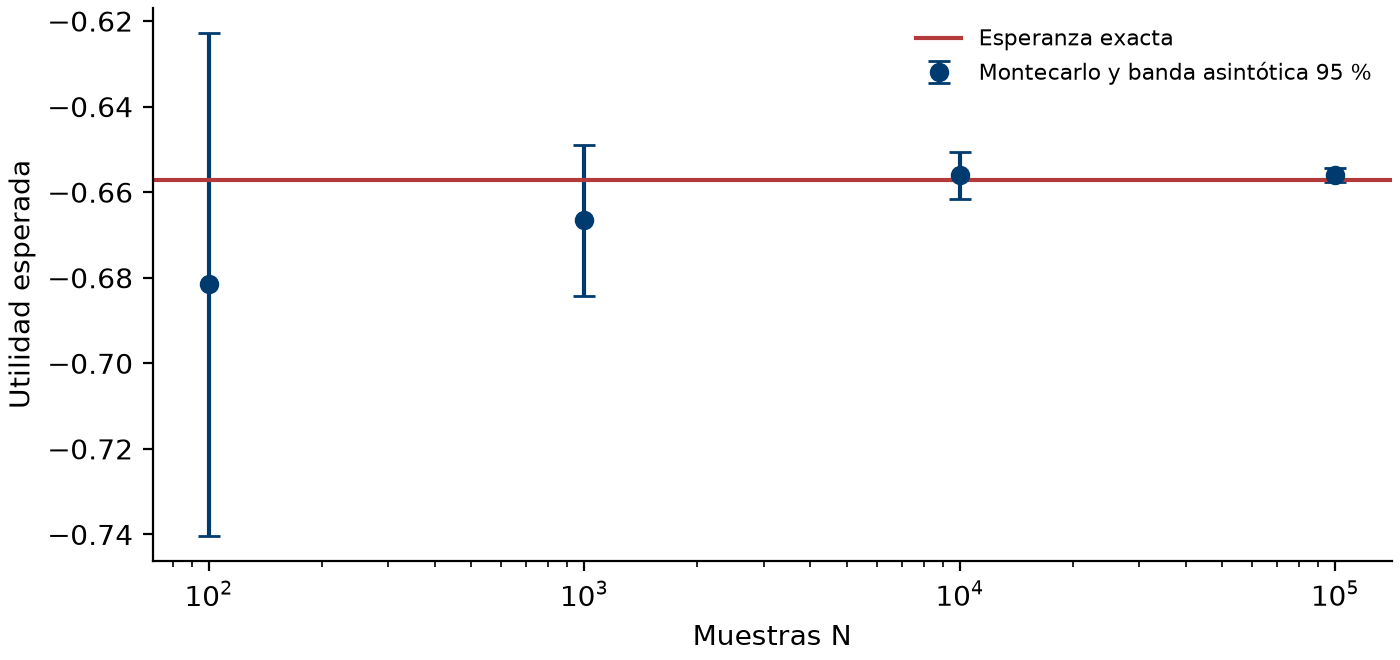
\includegraphics[height=.68\textheight]{figuras/integracion/montecarlo.png}\end{center}
Las bandas son intervalos asintóticos para la esperanza, no intervalos de predicción
para el consumo de un hogar.
\end{frame}

\begin{frame}{Gauss y Montecarlo en este ejemplo}
\begin{center}\begin{tabular}{lll}\toprule
Método&Evaluaciones&Error absoluto observado\\\midrule
Gauss--Hermite&8&$\approx3\times10^{-16}$\\
Montecarlo&100000&$1.0550\times10^{-3}$\\\bottomrule
\end{tabular}\end{center}
La ventaja de Gauss aquí depende de la suavidad, la dimensión uno y el peso normal conocido.
Montecarlo resulta útil cuando el integrando depende de muchas variables
o el modelo se dispone como un simulador.
Una comparación justa debe incluir costo por evaluación y generación de muestras.
\end{frame}

\begin{frame}{Integración en dimensión alta}
En un rectángulo $R\subset\R^d$, con $U$ uniforme en $R$,
\[\int_R f(x)\,dx=\operatorname{vol}(R)\mathbb E[f(U)].\]
Una regla producto con $m$ nodos por coordenada usa $m^d$ evaluaciones.
Montecarlo usa $N$ muestras y mantiene la escala $N^{-1/2}$ si hay varianza finita.
\begin{block}{Dependencia de la dimensión}
El exponente no depende de $d$, pero la varianza del integrando y el costo de
simular cada punto sí pueden crecer con la dimensión.
\end{block}
\end{frame}

\begin{frame}{Errores que conviene separar}
\begin{itemize}
\item \textbf{Modelo:} la demanda, la inversión o la distribución elegida pueden
no describir los datos económicos.
\item \textbf{Discretización:} una cuadratura o una malla temporal introduce error numérico.
\item \textbf{Muestreo:} Montecarlo introduce incertidumbre por simulación finita.
\item \textbf{Redondeo:} todas las implementaciones trabajan con precisión finita.
\end{itemize}
Un buen diagnóstico identifica qué error está estimando cada cifra reportada.
\end{frame}

\begin{frame}{Elección del procedimiento}
\small
\begin{center}\begin{tabular}{p{.43\linewidth}p{.48\linewidth}}\toprule
Situación&Procedimiento inicial\\\midrule
Tabla de datos&Trapecio; Simpson si la malla y regularidad lo justifican\\[1mm]
Función suave en una dimensión&Gauss o cuadratura adaptativa\\[1mm]
Esperanza con peso normal conocido&Gauss--Hermite con normalización correcta\\[1mm]
Trayectoria definida por una EDO&Forma integral y método de paso\\[1mm]
Simulación o muchas variables&Montecarlo con error estándar y diagnóstico de varianza\\\bottomrule
\end{tabular}\end{center}
La elección depende de qué evaluaciones están disponibles, del dominio y del error requerido.
\end{frame}

\begin{frame}{Actividades de cierre}
\begin{enumerate}
\item Compare los cocientes de error de Euler y trapecio al refinar la malla.
\item Repita Montecarlo con otras semillas. Distinga error observado y error estándar.
\item Calcule por Montecarlo $\int_0^{20}p(q)\,dq$ y el excedente de la primera clase.
\item Explique cuándo la aparente concordancia entre dos aproximaciones
puede ser insuficiente para afirmar que una integral está bien calculada.
\end{enumerate}
\end{frame}

\begin{frame}{Fuentes y cierre del bloque}
\small
\begin{itemize}
\item Sílabo 2026-2: integración y ecuaciones diferenciales vistas como ecuaciones integrales.
\item Material del curso: capítulos 7 y 8; complementos de cuadratura gaussiana.
\item NumPy: \href{https://numpy.org/doc/stable/reference/random/generator.html}{Generator y generación de números aleatorios}.
\item SciPy: \href{https://docs.scipy.org/doc/scipy/reference/integrate.html}{integración y problemas de valor inicial}.
\end{itemize}
Las tres clases comparten el cuaderno \texttt{Integracion\_Numerica\_2026-2.ipynb}.
La siguiente unidad del programa es optimización numérica.
\end{frame}

\end{document}
